% arara: pdflatex: { synctex: yes }
% arara: makeindex: { style: ctuthesis }
% arara: bibtex

% The class takes all the key=value arguments that \ctusetup does,
% and a couple more: draft and oneside
\documentclass[twoside]{ctuthesis}
\usepackage{graphicx}
\usepackage{listings}
\usepackage{mathtools}
\usepackage{caption}
\usepackage{subcaption}
\usepackage{matlab-prettifier}
\raggedbottom % This prevents text from sticking to the bottom of pages! Finally!


\ctusetup{
%	preprint = \ctuverlog,
	mainlanguage = english,
%	titlelanguage = czech,
%	mainlanguage = czech,
	otherlanguages = {czech},
	title-czech = {},
	title-english = {Use of Nintendo Wii balance boards with variable positioning during the Romberg test},
	subtitle-czech = {},
	subtitle-english = {\textit{Semester Project}},
	doctype = B,
	faculty = F7,
	department-czech = {Department in Czech},
	department-english = {Department of Biomedical Technology},
	author = {Noa Bar},
	supervisor = {Ing. Petr Volf},
	supervisor-address = {},
	fieldofstudy-english = {Biomedical technician},
	subfieldofstudy-english = {Biomedical and clinical technology},
	fieldofstudy-czech = {},
	subfieldofstudy-czech = {},
	keywords-czech = {},
	keywords-english = {Balance, Nintendo Wii Balance Board, Romberg test, Posture, Matlab Algorithm, Biomechanics},
	day = 20,
	month = 1,
	year = 2019,
	specification-file = {ctutest-zadani.pdf},
%	front-specification = true,
%	front-list-of-figures = false,
%	front-list-of-tables = false,
%	monochrome = true,
%	layout-short = true,
}

\ctuprocess

\addto\ctucaptionsczech{%
	\def\supervisorname{Vedoucí}%
	\def\subfieldofstudyname{Studijní program}%
}

\ctutemplateset{maketitle twocolumn default}{
	\begin{twocolumnfrontmatterpage}
		\ctutemplate{twocolumn.thanks}
		\ctutemplate{twocolumn.declaration}
		\ctutemplate{twocolumn.abstract.in.titlelanguage}
		\ctutemplate{twocolumn.abstract.in.secondlanguage}
		\ctutemplate{twocolumn.tableofcontents}
		\ctutemplate{twocolumn.listoffigures}
	\end{twocolumnfrontmatterpage}
}

% Theorem declarations, this is the reasonable default, anybody can do what they wish.
% If you prefer theorems in italics rather than slanted, use \theoremstyle{plainit}

\theoremstyle{plain}
\newtheorem{theorem}{Theorem}[chapter]
\newtheorem{corollary}[theorem]{Corollary}
\newtheorem{lemma}[theorem]{Lemma}
\newtheorem{proposition}[theorem]{Proposition}

\theoremstyle{definition}
\newtheorem{definition}[theorem]{Definition}
\newtheorem{example}[theorem]{Example}
\newtheorem{conjecture}[theorem]{Conjecture}

\theoremstyle{note}
\newtheorem*{remark*}{Remark}
\newtheorem{remark}[theorem]{Remark}

%\setlength{\parskip}{5ex plus 0.2ex minus 0.2ex}

% Abstract in Czech
\begin{abstract-czech}

\end{abstract-czech}

% Abstract in English
\begin{abstract-english}
 As balance and posture problems can be a sign of other medical conditions, as well as affect the day to day routine of people who suffer from them, it is important to keep watch for signs of balance deterioration.\\
 The drive of this project was to create an algorithm which will collect data from Nintendo Wii platforms, analyze it, and provide us with useful results to study in order to gain more knowledge about the subjects balance.\\
 The experiment consist of performing the Romberg test once with open eyes and again with closed eyes while standing on two Nintendo Wii Balance Boards. The data is collected then and statistically analyzed by a customized algorithm which was built specifically for the purpose of translating the weight data of the subjects into clear visual representations of their respective center of gravity, as well as the center of pressure for each foot.\\
 The visualization of the results allows the user of the software to clearly see the difference between maintaining balance with open eyes compared to closed eyes.
\end{abstract-english}

% Acknowledgements / Podekovani
\begin{thanks}
I would like to thank my supervisor Ing. Petr Volf for his support, advices, and help in conducting of the experiments.%\emph{alma mater}.
\end{thanks}

% Declaration / Prohlaseni
\begin{declaration}
 
I hereby declare that I have completed this semester project with the topic "Use of Nintendo Wii balance boards with variable positioning during the Romberg test" independently and I have included a full list of used references. \\

\vspace{5mm} % a small space between both paragraphs

I do not have a compelling reason against the use of the thesis within the meaning of Section 60 of the Act No 121/2000 Coll., on copyright, rights related to copyright and amending some laws (Copyright Act).\\

In Kladno,\ctufield{day}.~\monthinlanguage{title}~\ctufield{year}

\end{declaration}

% Only for testing purposes
\listfiles
\usepackage[pagewise]{lineno}
\usepackage{lipsum,blindtext}
\usepackage{mathrsfs} % provides \mathscr used in the ridiculous examples

\begin{document}

\maketitle

\section{Introduction}

Equilibrium is defined as a state in which all of the acting forces cancelled by each other, resulting in a stable, balanced system\cite{Physio}.\\
The maintenance of a stable posture in humans is possible due to the subsystems in our body which make up the postural control system.\\
Those subsystems are the Sensory system, which includes the visual and proprioceptive systems, the Central nervous system (CNS), and the muscle – skeletal system\cite{Control}.\\\par

Any disturbance in each of those subsystems can result in balance problems, which can be a result of old age, when balance control tend to degenerates\cite{Control}, as well as of many health conditions and medical procedures such as dizziness, too low or high blood pressure, result of head injury or a stroke, or as a result of neurological surgery for example\cite{Healthline}, and can greatly affect the daily life of the patients, when the fear of falling which might result in injury accompany daily activities such as standing up or walking\cite{Control}. Also, a change in a patient's usual balance can indicate the existing of an undiagnosed health problem like ear infection, unbalanced chemicals in the brain or even a tumor (acoustic neuroma)\cite{Healthline}.\\
Existing treatments includes medication, physical therapy, exercises at home and even surgery if needed \cite{Healthline}, and the sooner the change is detected – the better treatment the patient can get \cite{Gait}.\\\par

For those reasons it is important to measure the balance of a patient on a regular basis, but as for today, each existing mean have their own pros and cons; 
Scales, such as the Berg Balance scale, are the more common way to measure balance. But while cheaper and easy to use, they are not so accurate or sensitive to small changes, and have measurements limitations\cite{Gait}. \\
Therefore, in special medical facilities for gait and posture for example, it will be more common to find force platforms (FP), which in turn are more accurate and sensitive than a regular scale, but also expensive, not easy to set up, heavy and hard to transport, and as a result not so common in the average medical facilities\cite{Gait}.\\ 
Existing research\cite{Gait}found that if not as precise as the FP, especially in cases where extreme momentum involved, the results measured from Nintendo Wii Balance Boards (WBB) are similar enough to the results obtained from the FP to consider using the WBB as a reliable, easy to access, cheaper and portable way to measure balance in standard, non-specialist clinics, allowing better monitoring of the patient's balance over time and an improved detection of balance changes.\\\par   

While the Nintendo WBB can be a good solution for measuring balance in non-specialized medical facilities, exist a need for a platform which will be a clear and easy way to connect to WBB to computer, analyze the data, and give understandable results, in order to start utilizing them


\subsection{Aim of the project}
The aim of this project is to create an algorithm in Matlab which, when the software is connected to a pair of Nintendo Wii Balance Boards, could use the received data from the measurements and by calculating different parameters such as the center of pressure and center of gravity, will assess the standing balance of the person standing on them, giving an accurate report of their current balance condition.

\pagebreak

\section{List of abbreviations}
\begin{table}[H]
	\centering
	\begin{tabular}{|c|c|c|}
		\hline
		Abbreviation & Meaning & Unit \\ \hline
		COG & Center of Gravity & -\\
		COP & Center of Pressure & -\\
		FP & Force Platform & -\\
		S.D & Standard Deviation & -\\
		SW & Software & -\\
		WBB & Wii Balance Board & -\\
		\hline
	\end{tabular}
	\caption{List of used abbreviations}
\end{table}

\pagebreak

\begingroup
\renewcommand{\cleardoublepage}{}
\renewcommand{\clearpage}{}
\chapter{Methods}
\endgroup

In this project, a Matlab algorithm was created and used to collect and analyze the data acquired from performing a Romberg test on subjects standing on a pair of Nintendo Wii balance board platforms. 

\section*{Subjects}
This project uses measurements from 5 subjects; 3 males and 2 females, aged 25-35. All of the subjects were all normal volunteers, both students and employees from the FBME faculty in Kladno, Czech Republic, which personally agreed to take part in the measurements.

\begin{table}[H]
	\centering
	\begin{tabular}{| c |c|c| c|}
		\hline
		Subject number & Sex & Height (m) & Shoes type\\ \hline
		1 & F & 1.76 & Boots - flat soles\\
		2 & M & 1.83 & Snickers - flat soles\\
		3 & F & 1.52 & Boots - Platform, inner heels with even soles\\
		4 & M & 1.79 & Sport shoes - flat soles\\
		5 & M & 1.65 & Snickers - flat soles\\
		\hline
	\end{tabular}
	\caption{Test subjects details}
\end{table}

\section{Equipment}

\begin{itemize}
	\item Matlab R2018a (MathWorks, Massachusetts, United States)
	\item Two Nintendo Wii Balance Boards RVL-021 (Nintendo Co. Ltd., Japan)
\end{itemize}

\subsection{Calibration}
For calibration, the offsets of both platforms were taken and then subtract from each platform accordingly before the subject's measuring process begun
\pagebreak
\subsection{Equipment Set-up}
\begin{enumerate}
	\item The two Balance boards are positioned next to each other, with a 77 mm gap between them. 
	\item The dimensions of each platform are:
	\begin{itemize}
		\item Width = 238 mm
		\item Length = 433 mm
	\end{itemize}
\end{enumerate}

\begin{figure}[H]
	\centering
	\includegraphics[scale = 0.15]{Platform_Close}
	\caption{Wii Balance Boards set up}
\end{figure}


\section{Measurement procedure}
\subsection{Complications during the procedure}
While working on the software, there were unforeseen complications, for example, I could not get my computer to work with the libraries that connect between the platforms and the computer, no matter what I have tried – working with different versions of Matlab, trying different . Net frameworks or working from another computer with different Bluetooth driver, nothing solve it and I kept getting the following error code – 0xe0434352.\\
As this is a technical problem, I had agreed with my supervisor to temporarily using his laptop, and was able to perform the measurements I needed.\\
I believe that the problem could be due to a difference of windows versions; while I've tried to work with windows 8 and windows 10, my supervisor have windows 7 on his laptop, and since the libraries I have tried to work with are dated to back to 2007\cite{Error}, they might not work well with later version of windows.

\subsection{Romberg's test}
In order to perform the Romberg test (more about it in Appendix 1), the subject is asked to stand on the platforms – left leg at the center of the left platform and right leg at the center of the right platform, hands are relaxed at the sides of the body, head is at an upright position, looking forward, the subject is then asked to focus their stare on a marker sign, positioned at eye level for each subject and distanced 1.5 meter from the platforms' center.\\
The subject's data is then collected in two cycles of measurements, each time for 60 seconds – first cycle with eyes open, and second with eyes closed.\\

\begin{figure}[H]
	\centering
	\includegraphics[scale = 0.05]{FullBody}
	\caption{Subject position on the balance boards during the Romberg test}
\end{figure}

\subsection{Data Collection}
The platforms are connected to a computer via a Bluetooth connection, allowing the software to receive data from the 8 sensors located at the corners of each platform.\\
The data from the sensors is sampled for 60 seconds, at a sampling frequency of 30 Hz, making each measurement cycle yield 1,800 samples from the platforms sensors.\\ 
Those samples are then processed by a designated Matlab script, which computes the subject's center of pressure (CoP) and center of gravity (CoG) from the retrieved data.

\subsection{Methods for Data Analysis}
After receiving the left and right CoP and CoG calculated data from each sample, the code is then analyzing it, calculating the Mean, Median and Standard deviation of the different data x and z coordinates, visualizing the information and allowing a recognition of trends and changes.\\
Another tool used for analyzing the received data is measurements of the Euclidean distance between each point in the vector in order to see how stable on their feet the subject was during both of the tests, the code also calculate the mean and standard deviation of the result, in order to get a better picture of the information. 

\pagebreak

\begingroup
\renewcommand{\cleardoublepage}{}
\renewcommand{\clearpage}{}
\chapter{Measurement Results}
\endgroup
The following graphs details the results of the measurements taken, and help us visualize the subjects COP, COG, and their distribution over the course of the measurement. \\ 
The tables depict statistical analysis provided by the algorithm. COP measurements are in relation to each independent board, while the COG measurements are in relation to a unified coordinate system including both boards. In essence, COP (0,0) is the center of the relevant board, while COG (0,0) is the middle point between the two boards, i.e the center of the test set-up.

\section{Subject No. 1}

\begin{figure}[H]
	\centering
	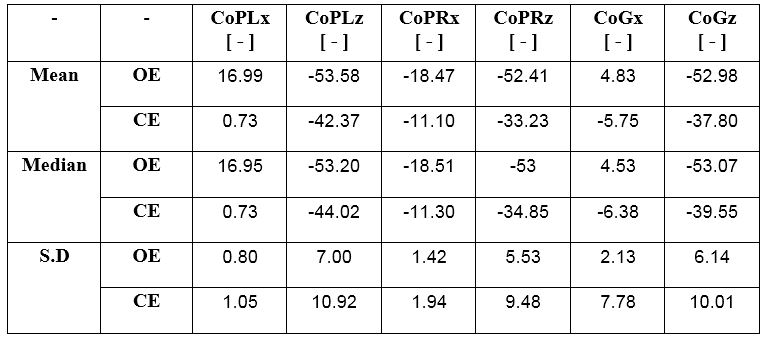
\includegraphics[width = \textwidth]{Patient1DataTable}
	\begin{table}[H]
		\caption{Mean, Median, and S.D of subjects measurements - closed vs open eyes}
	\end{table}
\end{figure}

\begin{figure}[H]
	\centering
	\begin{subfigure}{\textwidth}	
		\hspace*{-2cm}
		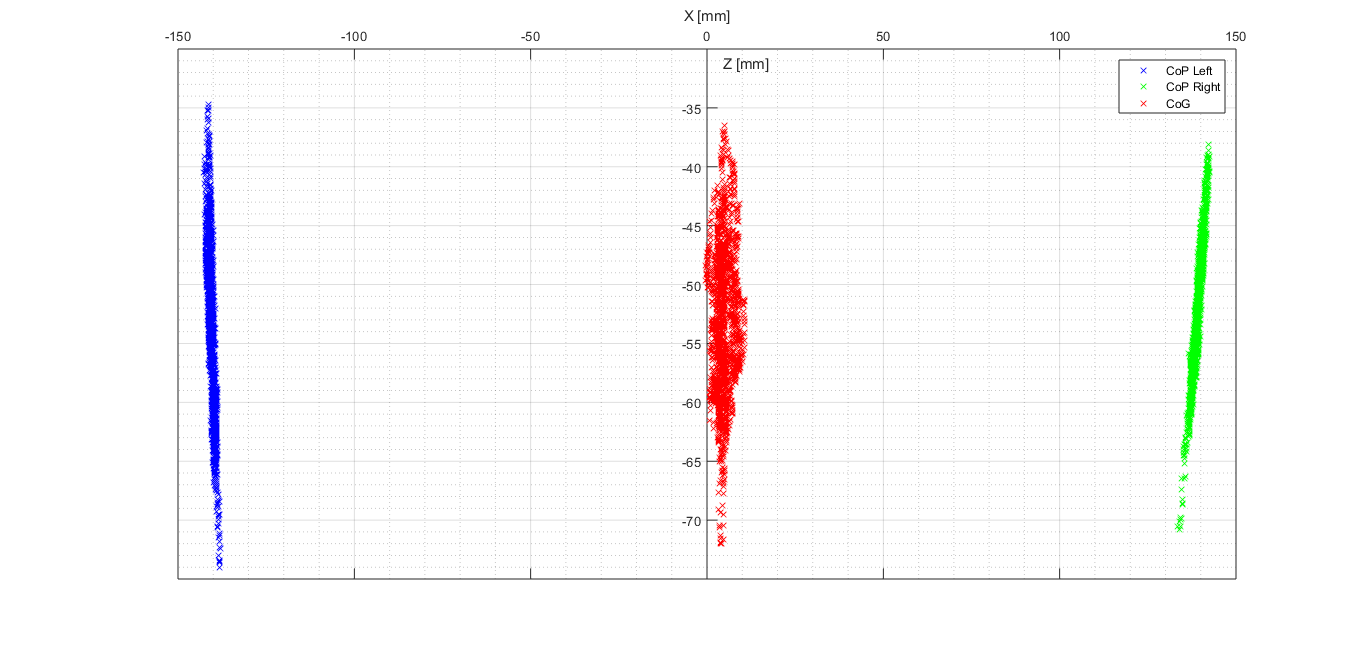
\includegraphics[scale=.45]{sub1_OE}
		\captionof{figure}{Left and Right COP measurements and COG measurement, Subject standing with open eyes}
	\end{subfigure}\hfil
	\begin{subfigure}{\textwidth}
		\hspace*{-2cm}
		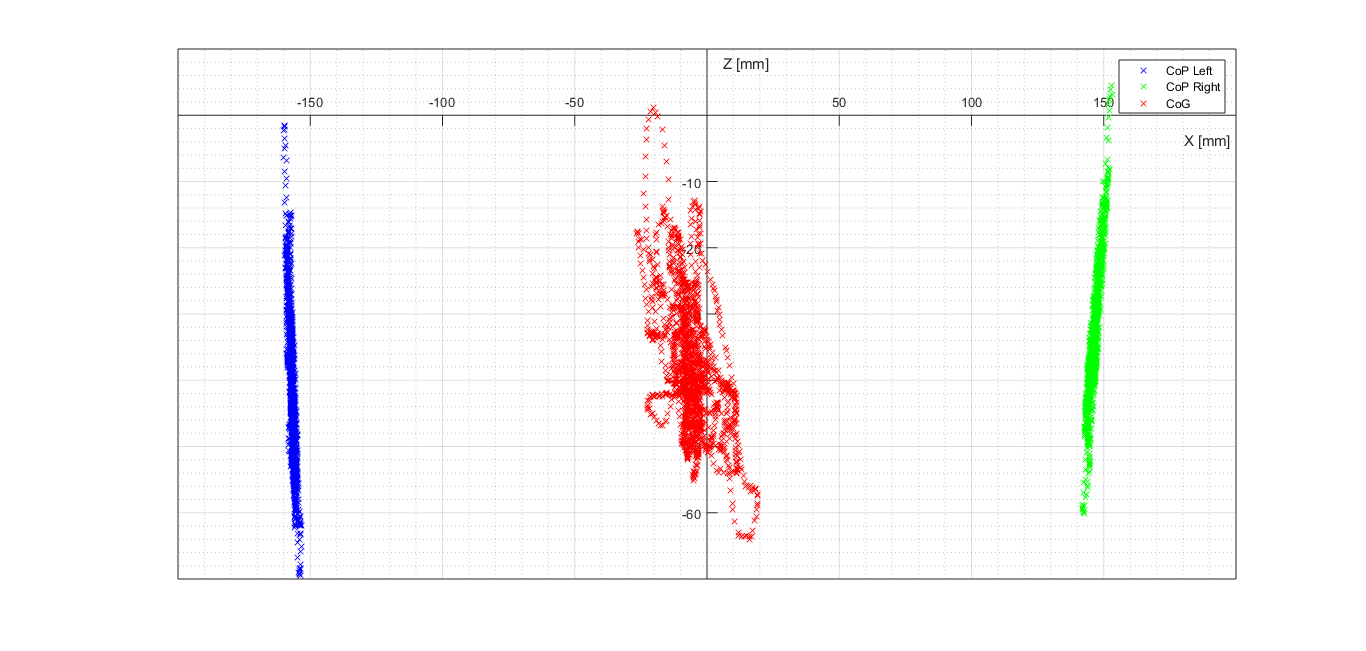
\includegraphics[scale=.45]{sub1_CE}
		\captionof{figure}{Left and Right COP measurements and COG measurement, Subject standing with closed eyes}
	\end{subfigure}
	\caption{COP and COG measurements of Subject No.1}
\end{figure}

\begin{figure}[H]
	\centering
	\begin{subfigure}{\textwidth}
		\hspace*{-1cm}
		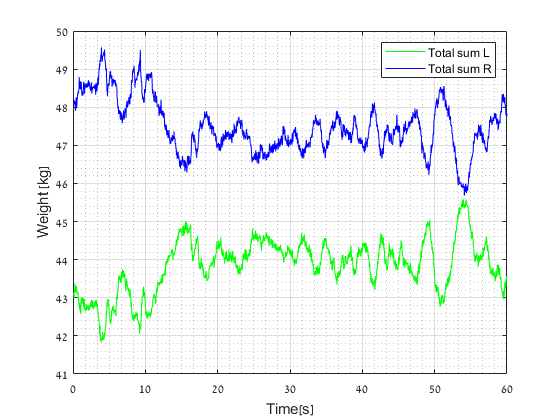
\includegraphics[scale=.9]{W_sub1_OE}
		\captionof{figure}{Weight distribution, open eyes}
	\end{subfigure}\hfil
	\begin{subfigure}{\textwidth}
		\hspace*{-1cm}
		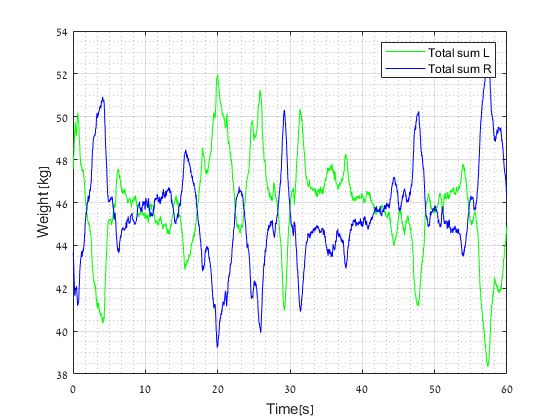
\includegraphics[scale=.9]{W_sub1_CE}
		\captionof{figure}{Weight distribution, closed eyes}
	\end{subfigure}
	\caption{Weight distribution of Subject No.1}
\end{figure}

\begin{figure}[H]
	\centering
	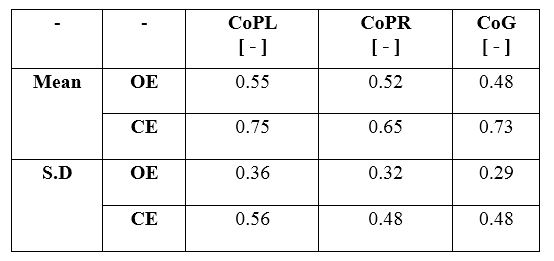
\includegraphics[width = 0.8\textwidth]{Patient1DistTable}
	\begin{table}[H]
		\caption{Mean, Median, and S.D of Euclidean distance between the points in each vector}
	\end{table}
\end{figure}


\section{Subject No. 2}

\begin{figure}[H]
	\centering
	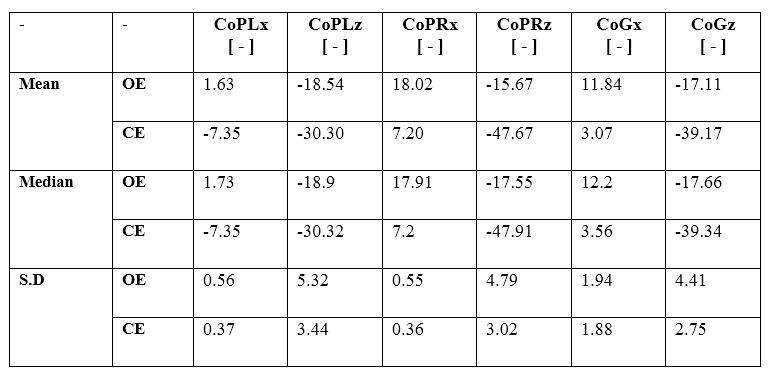
\includegraphics[width = \textwidth]{Patient2DataTable}
	\begin{table}[H]
		\caption{Mean, Median, and S.D of subjects measurements - closed vs open eyes}
	\end{table}
\end{figure}

\begin{figure}[H]
	\centering
	\begin{subfigure}{\textwidth}	
		\hspace*{-2cm}
		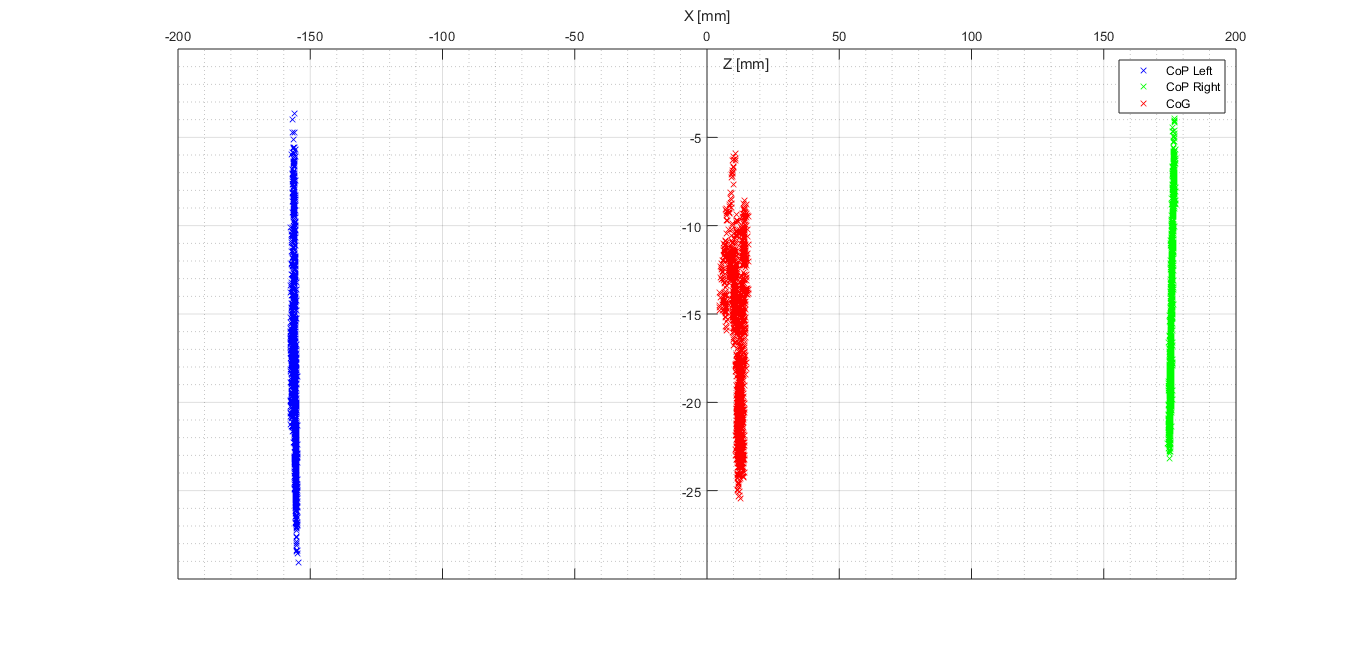
\includegraphics[scale=.45]{sub2_OE}
		\captionof{figure}{Left and Right COP measurements and COG measurement, Subject standing with open eyes}
	\end{subfigure}\hfil
	\begin{subfigure}{\textwidth}
		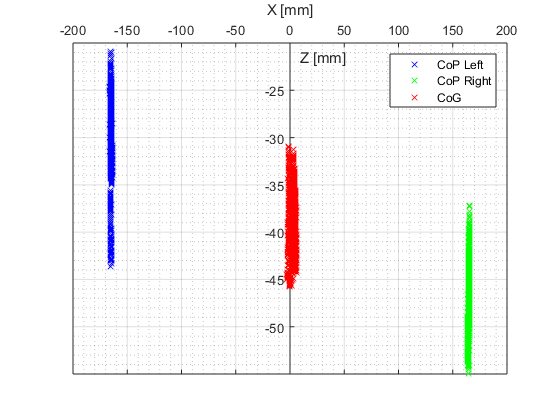
\includegraphics[scale=.9]{sub2_CE}
		\captionof{figure}{Left and Right COP measurements and COG measurement, Subject standing with closed eyes}
	\end{subfigure}
	\caption{COP and COG measurements of Subject No.2}
\end{figure}

\begin{figure}[H]
	\centering
	\begin{subfigure}{\textwidth}
		\hspace*{-1cm}
		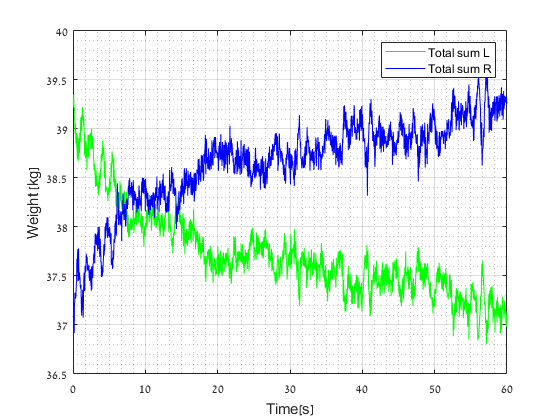
\includegraphics[scale=.9]{W_sub2_OE}
		\captionof{figure}{Weight distribution, open eyes}
	\end{subfigure}\hfil
	\begin{subfigure}{\textwidth}
		\hspace*{-1cm}
		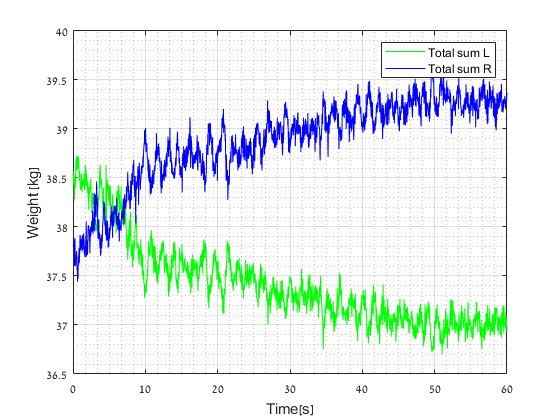
\includegraphics[scale=.9]{W_sub2_CE}
		\captionof{figure}{Weight distribution, closed eyes}
	\end{subfigure}
	\caption{Weight distribution of Subject No.2}
\end{figure}

\begin{figure}[H]
	\centering
	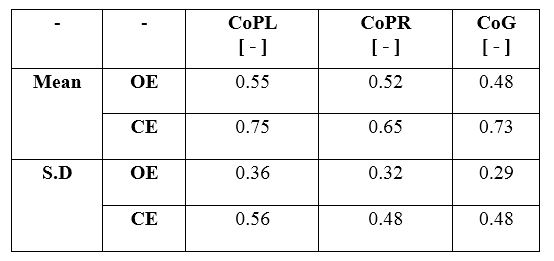
\includegraphics[width = .8\textwidth]{Patient1DistTable}
	\begin{table}[H]
		\caption{Mean, Median, and S.D of Euclidean distance between the points in each vector}
	\end{table}
\end{figure}

\section{Subject No. 3}

\begin{figure}[H]
	\centering
	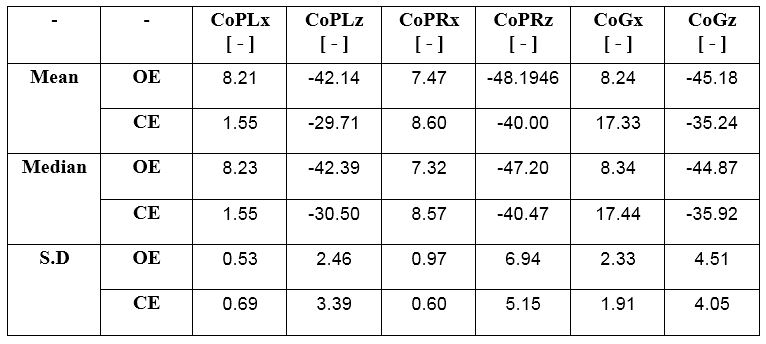
\includegraphics[width = \textwidth]{Patient3DataTable}
	\begin{table}[H]
		\caption{Mean, Median, and S.D of subjects measurements - closed vs open eyes}
	\end{table}
\end{figure}

\begin{figure}[H]
	\centering
	\begin{subfigure}{\textwidth}	
		\hspace*{-2cm}
		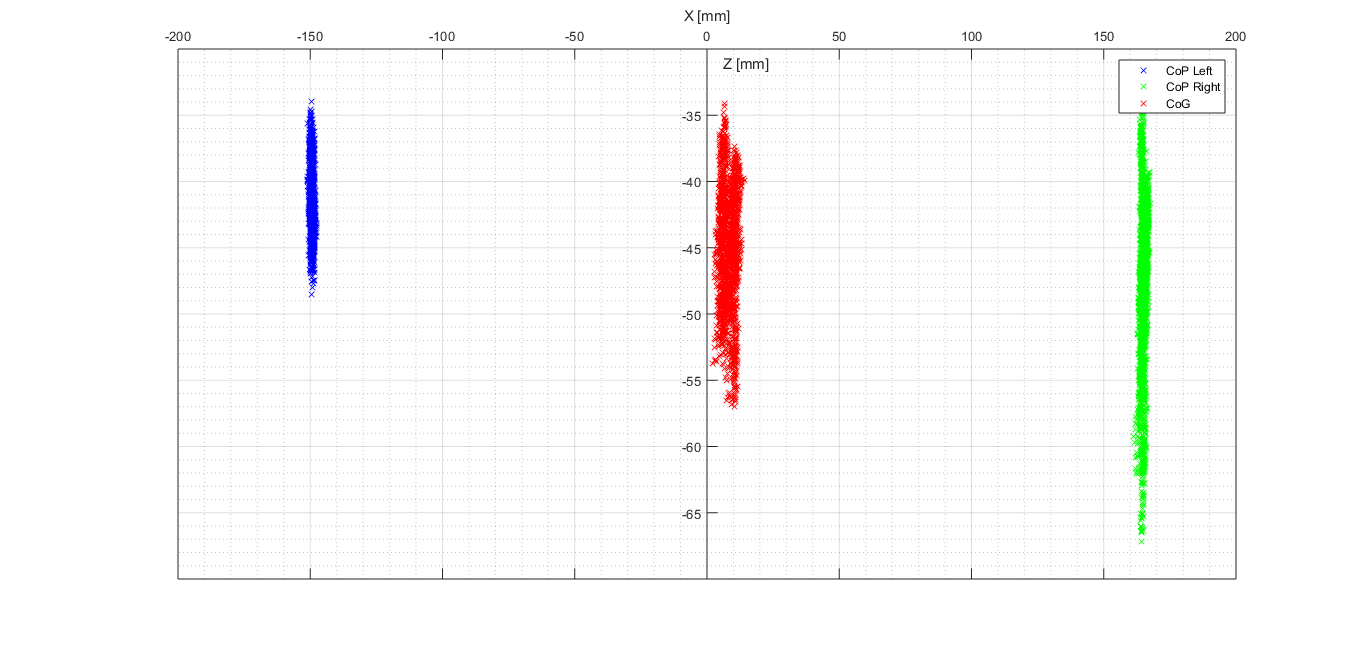
\includegraphics[scale=.45]{sub3_OE}
		\captionof{figure}{Left and Right COP measurements and COG measurement, Subject standing with open eyes}
	\end{subfigure}\hfil
	\begin{subfigure}{\textwidth}
		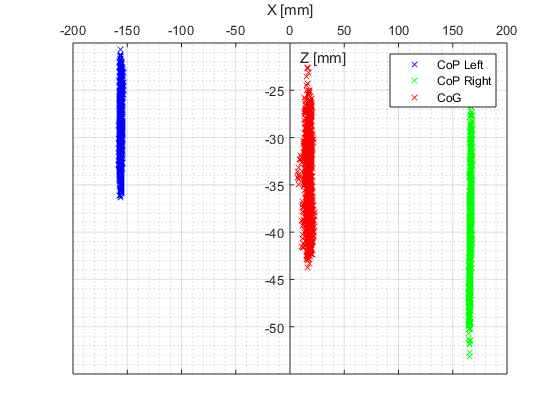
\includegraphics[scale=.9]{sub3_CE}
		\captionof{figure}{Left and Right COP measurements and COG measurement, Subject standing with closed eyes}
	\end{subfigure}
	\caption{COP and COG measurements of Subject No.3}
\end{figure}

\begin{figure}[H]
	\centering
	\begin{subfigure}{\textwidth}
		\hspace*{-1cm}
		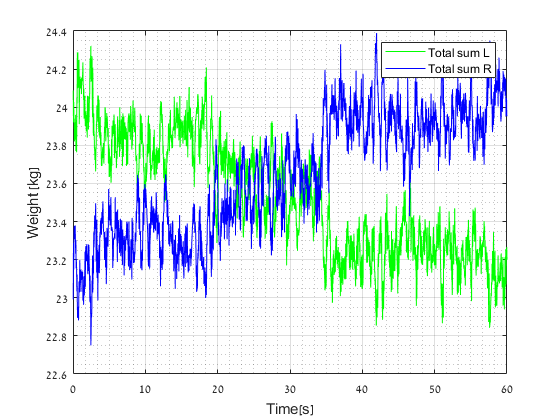
\includegraphics[scale=.9]{W_sub3_OE}
		\captionof{figure}{Weight distribution, open eyes}
	\end{subfigure}\hfil
	\begin{subfigure}{\textwidth}
		\hspace*{-1cm}
		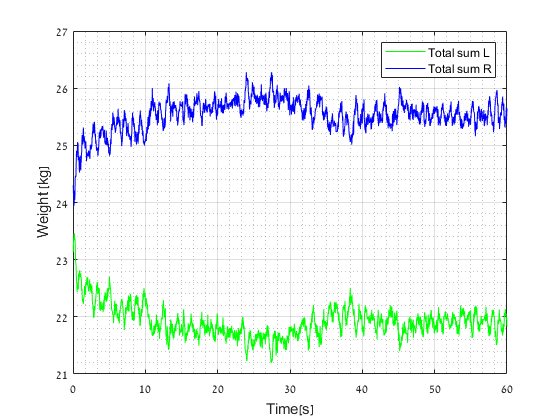
\includegraphics[scale=.9]{W_sub3_CE}
		\captionof{figure}{Weight distribution, closed eyes}
	\end{subfigure}
	\caption{Weight distribution of Subject No.3}
\end{figure}

\begin{figure}[H]
	\centering
	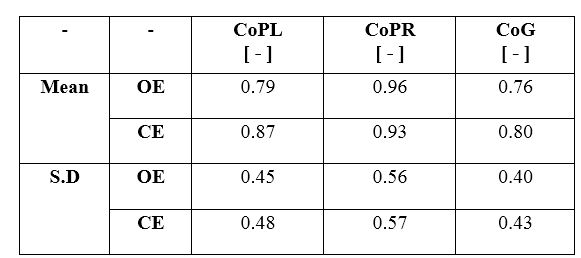
\includegraphics[width = .8\textwidth]{Patient3DistTable}
	\begin{table}[H]
		\caption{Mean, Median, and S.D of Euclidean distance between the points in each vector}
	\end{table}
\end{figure}

\section{Subject No. 4}

\begin{figure}[H]
	\centering
	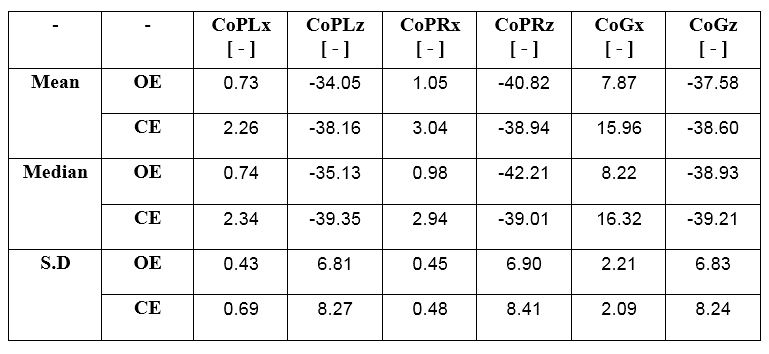
\includegraphics[width = \textwidth]{Patient4DataTable}
	\begin{table}[H]
		\caption{Mean, Median, and S.D of subjects measurements - closed vs open eyes}
	\end{table}
\end{figure}

\begin{figure}[H]
	\centering
	\begin{subfigure}{\textwidth}	
		\hspace*{-1cm}
		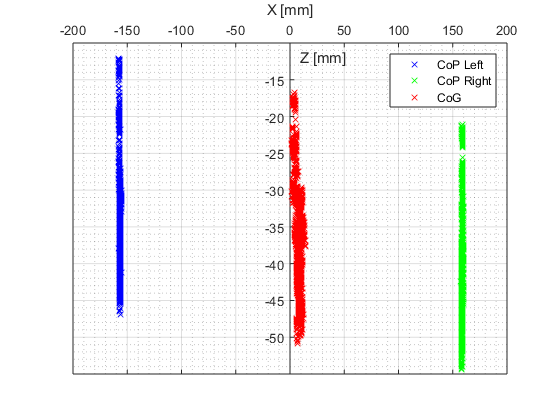
\includegraphics[scale=1]{sub4_OE}
		\captionof{figure}{Left and Right COP measurements and COG measurement, Subject standing with open eyes}
	\end{subfigure}\hfil
	\begin{subfigure}{\textwidth}
		\hspace*{-1cm}
		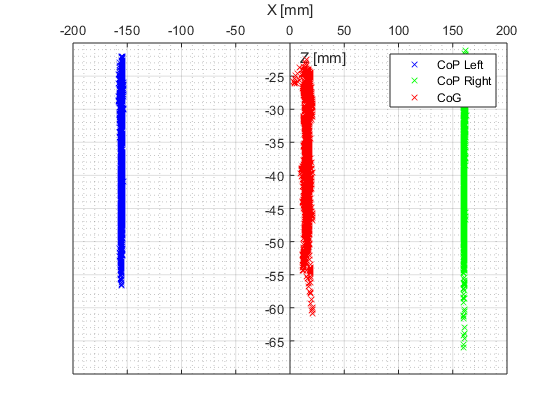
\includegraphics[scale=1]{sub4_CE}
		\captionof{figure}{Left and Right COP measurements and COG measurement, Subject standing with closed eyes}
	\end{subfigure}
	\caption{COP and COG measurements of Subject No.4}
\end{figure}

\begin{figure}[H]
	\centering
	\begin{subfigure}{\textwidth}
		\hspace*{-1cm}
		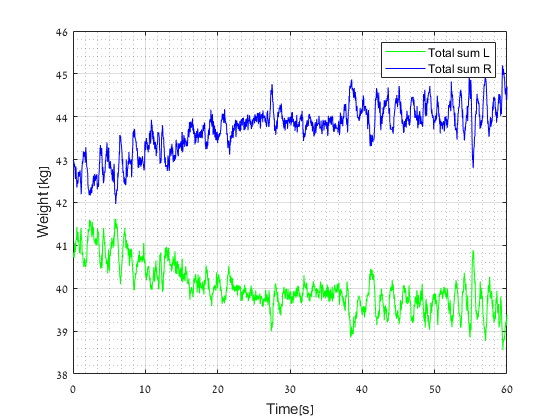
\includegraphics[scale=.9]{W_sub4_OE}
		\captionof{figure}{Weight distribution, open eyes}
	\end{subfigure}\hfil
	\begin{subfigure}{\textwidth}
		\hspace*{-1cm}
		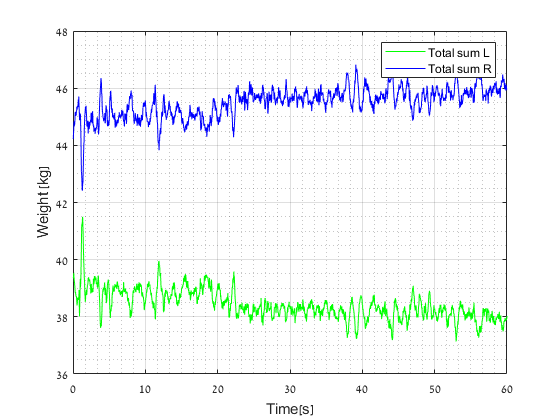
\includegraphics[scale=.9]{W_sub4_CE}
		\captionof{figure}{Weight distribution, closed eyes}
	\end{subfigure}
	\caption{Weight distribution of Subject No.4}
\end{figure}

\begin{figure}[H]
	\centering
	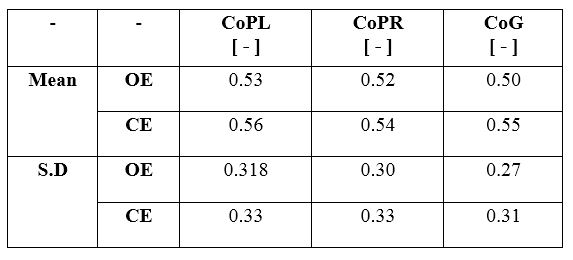
\includegraphics[width = .8\textwidth]{Patient4DistTable}
	\begin{table}[H]
		\caption{Mean, Median, and S.D of Euclidean distance between the points in each vector}
	\end{table}
\end{figure}

\section{Subject No. 5}

\begin{figure}[H]
	\centering
	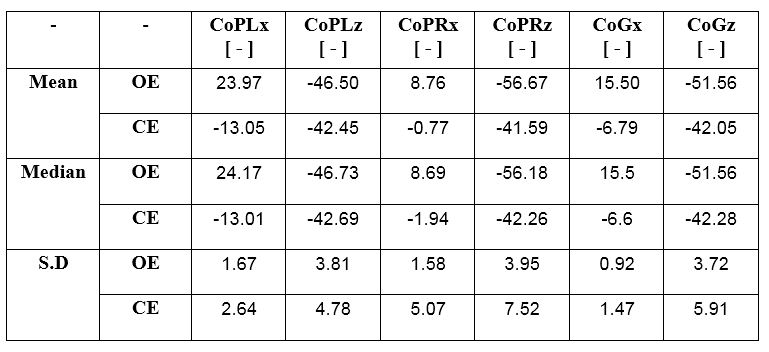
\includegraphics[width = \textwidth]{Patient5DataTable}
	\begin{table}[H]
		\caption{Mean, Median, and S.D of subjects measurements - closed vs open eyes}
	\end{table}
\end{figure}

\begin{figure}[H]
	\centering
	\begin{subfigure}{\textwidth}
		\hspace*{-1cm}	
		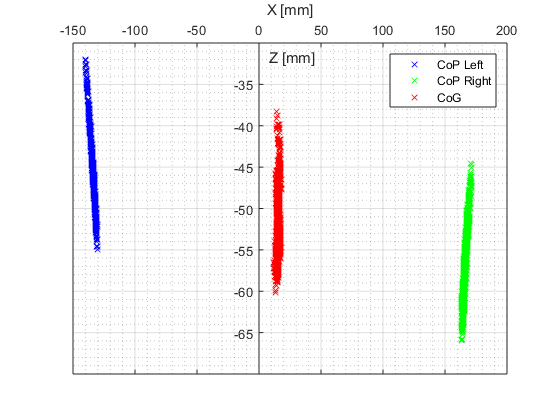
\includegraphics[scale=1]{sub5_OE}
		\captionof{figure}{Left and Right COP measurements and COG measurement, Subject standing with open eyes}
	\end{subfigure}\hfil
	\begin{subfigure}{\textwidth}
		\hspace*{-1cm}
		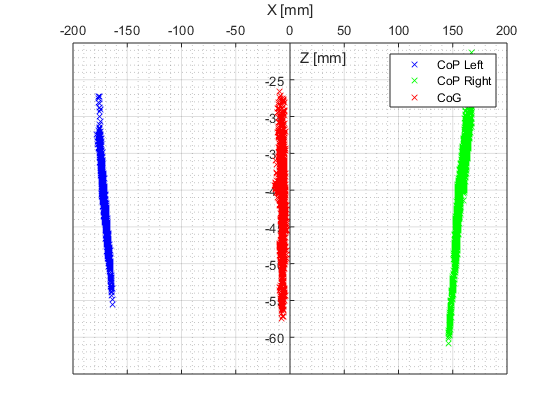
\includegraphics[scale=1]{sub5_CE}
		\captionof{figure}{Left and Right COP measurements and COG measurement, Subject standing with closed eyes}
	\end{subfigure}
	\caption{COP and COG measurements of Subject No.5}
\end{figure}

\begin{figure}[H]
	\centering
	\begin{subfigure}{\textwidth}
		\hspace*{-1cm}
		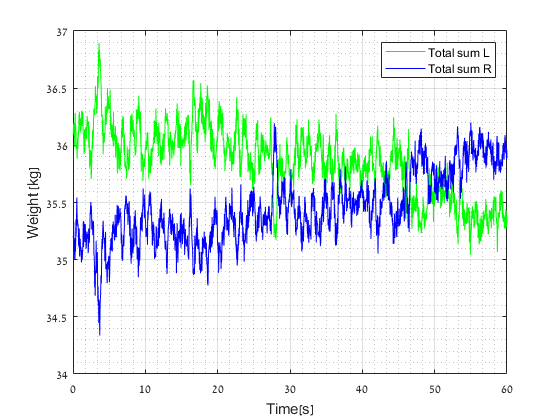
\includegraphics[scale=1]{W_sub5_OE}
		\captionof{figure}{Weight distribution, open eyes}
	\end{subfigure}\hfil
	\begin{subfigure}{\textwidth}
		\hspace*{-1cm}
		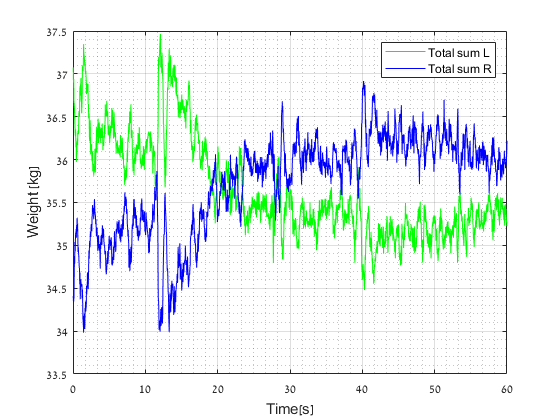
\includegraphics[scale=1]{W_sub5_CE}
		\captionof{figure}{Weight distribution, closed eyes}
	\end{subfigure}
	\caption{Weight distribution of Subject No.5}
\end{figure}

\begin{figure}[H]
	\centering
	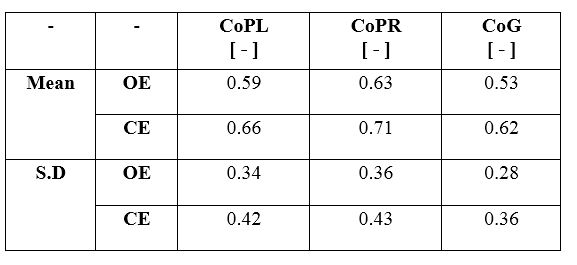
\includegraphics[width = .8\textwidth]{Patient5DistTable}
	\begin{table}[H]
		\caption{Mean, Median, and S.D of Euclidean distance between the points in each vector}
	\end{table}
\end{figure}


\pagebreak

\begingroup
\renewcommand{\cleardoublepage}{}
\renewcommand{\clearpage}{}
\chapter{Discussion}
\endgroup

This project was using the data collected from performing the Romberg test on 5 subject, and analyzing it with a code written in Matlab, in order to learn about the subjects balance.\\
While some subjects had better balance then others (subjects 2 and 4 for example), the findings were similar along the measurements, and showed some reoccurring trends.\\
It could be seen that through all the centers of pressure and center of gravity's S.D calculations that the S.D of the Z coordinates was larger than the S.D of the X coordinates, showing that the subjects' movements and swaying in order to keep balanced were mostly forwards and backwards on their feet, and not to the sides.\\
It can also be seen through most of the measurements that the S.D values of the closed eyes measurements were larger than the S.D values of the open eyes measurements, both in the CoP and CoG calculations, and in the Euclidean distance between the points in each vector. This part was expected, since closing eyes eliminates one of the three senses the body requires in order to maintain balance while standing - the vision\cite{Physio}. When all three of those senses are working correctly, the body should not have a problem to remain balanced and any swaying would be minimal. Without the sense of vision, however, the body will lose its balance more often and would have to work harder to keep itself balanced, leading to lager movements back and forth and back to the center again as the body attempts to compensate for the missing sense.\\
Another trend which could be seen from the observed data is the weight alternation between the feet during the test. While the eyes were open, it could be seen from the graphs (figures 15, 21 for example) that the weight is gradually shifted to one foot, usually the dominant one – the right foot in most subjects – a trend which seems to strengthen as time passes. Yet when the eyes are closed, the weight divides almost evenly between the feet and remains that way for the entire test (figures 16, 22 for example).\\
This could be due to the body's need to rely more on other balance mechanisms in order to maintain balance once the vision is eliminated. While dividing body weight equally on two feet can help to keep a sense of space and position, leaning on a single foot could lead to the body losing its balance and falling to the side.\\
During my work I have encountered a limitation that might affect the future using of the code, and would have to be fixed. As stated in the 'Measurements procedure' part in the methods section, the libraries I was trying to use in order to connect the platforms to a computer did not work on my laptop, and therefore I had to run my code and perform the measurements using my code on the laptop of professor Volf – this project's supervisor. This limitation needs to be resolved in order for the code to work on every computer.\\
The collected data and derived statistical analysis shows how much we can learn from testing a person's balance, and how important it is to have a way to follow and monitor this information.\\
The program was created to analyze the collected data, and could allow better monitoring of a person's balance over time and improve detection and treatment of balance changes, and can be expanded in the future for further analysis of the topic.\\

\pagebreak

\begingroup
\renewcommand{\cleardoublepage}{}
\renewcommand{\clearpage}{}
\chapter{Conclusion}
\endgroup

This project showed that the Nintendo Wii Balance boards can be an easy to transport and not expensive option to measure and keep track of people's balance, which can make the act of monitoring and recognizing balance issues on time easier, convenient, and cheaper.\\
I believe that the project can open a way to similar works in the future, focusing on more specific or different data which could be collected from analyzing a person's standing and balance.\\
I myself would try to use this code and platforms, combined with Kinect v2 cameras to examine the correlation between weight and center of pressure to spinal alignment as my thesis work in the future.


\appendix


\chapter{Romberg's test}

Romberg test is a clinical test, named after the German neurologist Moritz Heinrich Romberg (1795–1873), and was used for over 100 years to assess a person's neurological function of balance\cite{Physio}.\\ 
The test is based on the idea that while our body require 3 senses to keep itself balance while standing, 2 of them are enough to stay balanced, and are able to compensate the missing sense\cite{Physio}.\\ 
The senses are:\\ 
1. Proprioception – the ability to know your body position in space\\
2. Vestibular – the ability to know your head position in space\\
3. Vision – can be used to evaluate and adjust body position \\
\\
The test is checking if there is a problem related to the sense of proprioception, and since a person can still maintain balance based on the other two senses, the subjects in the test are asked to stand still and close their eyes. A healthy patient or a patient which their balance problems are from another source, would be able to maintain upright, using the other two senses – inability to maintain balance and falling down is considered a positive result in the Romberg test\cite{Physio}.\\ 
Having a positive result in the test can point that the patient's ataxia - loss of control of bodily movements – is from a sensory source, and related to the loss of proprioception. A negative result in the test tell us that the source of the ataxia is cerebellar in its nature in case of a patient with the medical condition\cite{Physio}.\\


\chapter{Matlab code to analyze the retrieved data from the Wii board} 

\begin{lstlisting}[style=Matlab-editor]
clc; clear all; close all;
%%%%%%%%%%%%%%%%%%%%%%%%%%%%%%%%%%%%%%%%%%%%%%%%%%%%%%%
%%%% Board connections
%%% This section was used to retrieve information from the platforms to
%%% professor Volf's laptop. It was commented out since parts of it cause 
%%% my Matlab to crash
%%%%%%%%%%%%%%%%%%%%%%%%%%%%%%%%%%%%%%%%%%%%%%%%%%%%%%%
% % bb1 = actxserver('WiiLab.WiiLAB');
% % bb1.Connect();
% % bb2 = actxserver('WiiLab.WiiLAB');
% % bb2.Connect();
% clearvars -except bb1 bb2
% OffsetL = bb1.GetBalanceBoardSensorState()/4;
% OffsetR = bb2.GetBalanceBoardSensorState()/4;
% i = 1;
% % Duration = 60 seconds;
% % Frequancy = 30 Hz;
% for j=1:1800;
% PlatformL(i,:) = (bb1.GetBalanceBoardSensorState()/4)-OffsetL;
% PlatformR(i,:) = (bb2.GetBalanceBoardSensorState()/4)-OffsetR;
% PlatformTime(i,:) = clock;
% i = i+1;
% pause(1/30);
% end
%%%%%%%%%%%%%%%%%%%%%%%%%%%%%%%%%%%%%%%%%%%%%%%%%%%%%%

% Board Parameters:
% Distance measurements and offsets in milimeters
%%%%%%
MatrixOfData = load('Proband5_CE.mat');
halfOfBoardLength = 433/2;
halfOfBoardWidth = 238/2;
distanceBetweenPlatforms = 77;
PlatformOffset = 157.5;% Distance from Total center to platform center (mm)

%%%%%%%%%%%%%%%%%%
% Retrieve data for plotting
%%%%%%%%%%%%%%%%%%

for n = 1:length(MatrixOfData.PlatformL(:,1))
% Left platform sensors data points
LPLT(n) = MatrixOfData.PlatformL(n,4);
LPLB(n) = MatrixOfData.PlatformL(n,3);
LPRT(n) = MatrixOfData.PlatformL(n,2);
LPRB(n) = MatrixOfData.PlatformL(n,1);

% Right platform sensors data points
RPLT(n) = MatrixOfData.PlatformR(n,1);
RPLB(n) = MatrixOfData.PlatformR(n,2);
RPRT(n) = MatrixOfData.PlatformR(n,3);
RPRB(n)= MatrixOfData.PlatformR(n,4);

% Calculate the sum of the sensors for each platform
totalSumOfSensorsLeft(n) = (LPLT(n)+LPLB(n)+LPRT(n)+LPRB(n));
totalSumOfSensorsRight(n) = (RPLT(n)+RPLB(n)+RPRT(n)+RPRB(n));

% Time
ClockTime(n) = MatrixOfData.PlatformTime(n,6);
end


%%%%%%%%%%%%%%%%%%
% Do the math
%%%%%%%%%%%%%%%%%%

% Set up vectors
CoPLeftX = [];
CoPLeftZ = [];
CoPRightX = [];
CoPRightZ = [];
CoGx = [];
CoGz = [];

% Calculate center of pressure and center of gravity
for m = 1:length(MatrixOfData.PlatformL(:,1))

% Center of pressure Left Board
[CoPLeftX(m), CoPLeftZ(m)] = centerOfPressureLeft(LPRB(m), LPRT(m), LPLB(m),...
LPLT(m),halfOfBoardLength, halfOfBoardWidth);

% Center of pressure on Right Board
[CoPRightX(m), CoPRightZ(m)] = centerOfPressureRight(RPLT(m), RPLB(m),RPRT(m),...
RPRB(m),halfOfBoardLength, halfOfBoardWidth);

% Center of gravity total
[CoGx(m), CoGz(m)] = centerOfGravity(LPRB(m), LPRT(m), LPLB(m), LPLT(m),...
RPLT(m), RPLB(m), RPRT(m),RPRB(m), CoPLeftX(m), CoPLeftZ(m), ...
CoPRightX(m), CoPRightZ(m), PlatformOffset);

% Set up matrix of results
MatrixOfResults(m,:) = [ClockTime(m),LPLT(m),LPLB(m),LPRT(m),LPRB(m),RPLT(m),...
RPLB(m), RPRT(m), RPRB(m), CoPLeftX(m), CoPLeftZ(m), CoPRightX(m),...
CoPRightZ(m),CoGx(m), CoGz(m)];

% Calculate distances between points in the vectors
if m == 1
continue
else
CoPDistL(m) = euclidDist(CoPLeftX(m-1),CoPLeftZ(m-1),CoPLeftX(m),...
CoPLeftZ(m));

CoPDistR(m) = euclidDist(CoPRightX(m-1),CoPRightZ(m-1),CoPRightX(m),...
CoPRightZ(m));

CoGDist(m) = euclidDist(CoGx(m-1),CoGz(m-1),CoGx(m),CoGz(m));
end
end

% Use the matrix to calculate statistical data
for n = 10:length(MatrixOfResults(1,:))
MeanOfColumns(n-9) = mean(MatrixOfResults(:,n));
MedianOfColumns(n-9) = median(MatrixOfResults(:,n));
StandardDeviarionOfColumns(n-9) = std(MatrixOfResults(:,n));
end 
%%%%%%%%%%%%%%%%%%%
%Calculate the means and standart deviation of the distance between data
%points
%%%%%%%%%%%%%%%%%%%

meanOfCoPDistL = mean(CoPDistL)
meanOfCoPDistR = mean(CoPDistR)
meanOfCoGDist = mean(CoGDist)

stdOfCoPDistL = std(CoPDistL)
stdOfCoPDistR = std(CoPDistR)
stdOfCoGDist = std(CoGDist)

%%%%%%%%%%%%%%%%%%
% Write data in Excel
%%%%%%%%%%%%%%%%%%
vectorHeader = {'Time','LPLT','LPLB','LPRT','LPRB','RPLT','RPLB','RPRT'...
,'RPRB','COPLx','COPLz','COPRx','COPRz','COGx','COGz'};
xlswrite('dataAnalyzerSheet.xlsx',vectorHeader,'A1:O1');
vectorSider = {'Mean','Median','S.D'};
xlswrite('dataAnalyzerSheet.xlsx',vectorSider(:),'I1804:I1806');
xlswrite('dataAnalyzerSheet.xlsx',MatrixOfResults,'A2:O1801');
xlswrite('dataAnalyzerSheet.xlsx',MeanOfColumns,'J1804:O1804');
xlswrite('dataAnalyzerSheet.xlsx',MedianOfColumns,'J1805:O1805');
xlswrite('dataAnalyzerSheet.xlsx',StandardDeviarionOfColumns,'J1806:O1806');

% Open Excel file
winopen('dataAnalyzerSheet.xlsx')


%%%%%%%%%%%%%%%%%%
%Plotting
%%%%%%%%%%%%%%%%%%
figure(1)
ax = gca;
plot(CoPLeftX - PlatformOffset,CoPLeftZ,'xb',CoPRightX + PlatformOffset,...
CoPRightZ,'xg',CoGx,CoGz,'xr')
legend('CoP Left','CoP Right','CoG')
ax.XAxisLocation = 'origin';
ax.YAxisLocation = 'origin';
xlabel('X [mm]');
ylabel('Z [mm]');
grid on
grid minor

samp = 1:1800;
figure(2)
ax = gca;
plot(samp,totalSumOfSensorsLeft,'g')
LineWidth = 0.5;
ax.XAxisLocation = 'origin';
ax.YAxisLocation = 'origin';
xlabel('Time[s]');
ylabel('Weight [kg]');
xticks(0:300:1800);
xticklabels([0:10:60]);
grid on
grid minor
hold on
plot(samp,totalSumOfSensorsRight,'b')
legend('Total sum L','Total sum R')

figure(3)
subplot(3,1,1)
ax = gca;
plot(samp,CoPDistL,'b', 'LineWidth', 0.5)
ax.XAxisLocation = 'origin';
ax.YAxisLocation = 'origin';
title('CoP Dist.Left')
line([0 samp(end)], [meanOfCoPDistL meanOfCoPDistL], 'LineWidth', 1,...
'Color', 'k')

subplot(3,1,2)
ax = gca;
plot(samp,CoPDistR,'g')
ax.XAxisLocation = 'origin';
ax.YAxisLocation = 'origin';
title('CoP Dist.Right')
line([0 samp(end)], [meanOfCoPDistR meanOfCoPDistR], 'LineWidth', 1,...
'Color', 'k')

subplot(3,1,3)
ax = gca;
plot(samp,CoGDist,'r')
ax.XAxisLocation = 'origin';
ax.YAxisLocation = 'origin';
title('CoG Distance')
line([0 samp(end)], [meanOfCoGDist meanOfCoGDist], 'LineWidth', 1,...
'Color', 'k')

%%%%%%%%%%%%%%%%%%
% Function definitions
%%%%%%%%%%%%%%%%%%
function [COPLx,COPLz] = centerOfPressureLeft(s1, s2, s3, s4, BParam1, BParam2)
% Calculates center of pressre of the Left Platform.
% Accepts data from four sensors and board parameters,  
% returns center of pressure X and center of pressure Z
FLtotal = s1 + s2 + s3 + s4; % Total force

momentOfInertiaLX = BParam1 * (-s1+s2-s3+s4);
momentOfInertiaLZ = BParam2 * (s1+s2-s3-s4);

COPLx = momentOfInertiaLZ/FLtotal;
COPLz = momentOfInertiaLX/FLtotal;

COPLx = round(COPLx,2);
COPLz = round(COPLz,2);
end

function [COPRx,COPRz] = centerOfPressureRight(s1, s2, s3, s4, BParam1, BParam2)
% Calculates center of pressre of the Right Platform.
% Accepts data from four sensors and board parameters,  
% returns center of pressure X and center of pressure Z
FRtotal = s1 + s2 + s3 + s4; % Total force

momentOfInertiaRX = BParam1 * (s1-s2+s3-s4);
momentOfInertiaRZ = BParam2 * (-s1-s2+s3+s4);

COPRx = momentOfInertiaRZ/FRtotal;
COPRz = momentOfInertiaRX/FRtotal;

COPRx = round(COPRx,2);
COPRz = round(COPRz,2);
end

function [COGx,COGz] = centerOfGravity(s1, s2, s3, s4, s5, s6, s7, s8, ...
COPLx, COPLz, COPRx, COPRz, offset)
% calculates coordinates of center of gravity
% Accepts info from sensors and COP coordinates
% Returns center of gravity X and center of gravity Z

% Offsets
xOffsetCOPL = COPLx - offset;
xOffsetCOPR = COPRx + offset;

% Weights from sensors
platformWeightLeft = s1 + s2 + s3 + s4;
platformWeightRight = s5 + s6 + s7 + s8;
platformsWeightTotal = platformWeightLeft + platformWeightRight;

% Moments of Inertia
xMomentLeft = platformWeightLeft * xOffsetCOPL;
xMomentRight = platformWeightRight * xOffsetCOPR;
zMomentLeft = platformWeightLeft * COPLz;
zMomentRight = platformWeightRight * COPRz;
xMomentTotal = xMomentLeft + xMomentRight;
zMomentTotal = zMomentLeft + zMomentRight;

% Center of gravity
COGx = xMomentTotal/platformsWeightTotal;
COGz = zMomentTotal/platformsWeightTotal;

COGx = round(COGx,2);
COGz = round(COGz,2);
end


% Euclidean distance between two points
function [dist] = euclidDist(x1, y1, x2, y2)
% Accepts two points with x,y coordinates and returns the euclidean 
% distance between them
dist = sqrt(((x2-x1)^2)+((y2-y1)^2));
end

\end{lstlisting}


\begin{thebibliography}{9}
	\bibitem{Gait}
	ROSS A. CLARCK ET EL. \textit{Validity and reliability of the Nintendo Wii Balance Board for assessment of standing balance.} Elsevier, Gait \& Posture 31 (2010) 307–310\\
	https://www.sciencedirect.com/science/article/pii/S096663620900664X
	
	\bibitem{Error}
	\uppercase{Cooper J, Siegfried K, Ahmed AA} (2014) \textit{BrainBLoX: Brain and Biomechanics Lab in a Box Software (Version 1.0)} [Software]
	
	\bibitem{Physio}
	\textit{Romberg's Test}, accessed on 12.11.2018, \textit{https://www.physio-pedia.com/Romberg\textunderscore Test}
	
	\bibitem{Control}
	\uppercase{Winter A. David, Et El.} \textit{Assessment of balance control in humans}, Academic publishers, Medical Progress Through Technology 16 (1990) 31-51\\
	
	\bibitem{Healthline}
	\uppercase{Chitra Badii, Marijane Leonard, MD William A Morrison} (2016) \textit{What Causes Poor Balance?}, accessed on 30.1.2019\\
	https://www.healthline.com/symptom/poor-balance
	
	
\end{thebibliography}



\ctutemplate{specification.as.chapter}

\end{document}
